\subsubsection*{Pickle Rick}
\addcontentsline{toc}{subsubsection}{Pickle Rick}
This Rick and Morty-themed challenge requires you to exploit a web server and find three ingredients to help Rick make his potion and transform himself back into a human from a pickle.\\

We are given no more instructions or help, since this is a room to check the learned knowledge of the previous rooms.\\
We proceed as follows: \\
First we run a Gobuster scan (as it takes longer than other scans) against the target, where we find the directories /assets with status code 301 and /server-status with status code 403.\\
Looking at the /assets website we only find some gifs and pictures we cannot make any use of as of now.\\

In the meantime, we take a look at the website's source code, build languages, etc., where we see that the website runs Ubuntu on an Apache server.\\
Either intercepting the loading of the page or plainly looking at the source code we find this note:
\cdnl{
    <!-$\,$- Note to self, remember username!Username: R1ckRul3s -$\,$->
}
Still, we don't have any login page or password to try it with.\\

We run an Nmap scan on the website and ``only'' find open ports 80 and 223,  which doesn't help us much either.\\

What we can try is to enumerate further with gobuster and look for any other sites and the most common site types , i.e activating the \cd{-x php,html,css,js,pdf,txt} switch on the gobuster scan.\\
This looks way more promising, since we then find the sites \cd{index.html, login.php, portal.php} and \cd{robots.txt}
Under \cd{login.php} we see a login site we cannot really exploit yet, so we take a look at the other sites.\\
\cd{portal.php} redirects us to the same login page we were in before.\\
In the page \cd{robots.txt} we only see the word \cd{Wubbalubbadubdub}, so in lack of anything better we try it as a password and see it works!\\
We land in the \cd{portal.php} site, where apparently there is a command line interface we find to work with Linux after some trials.\\
We note when loading this site that there is a comment encoded in Base64: 
\cdnl{<!-- Vm1wR1UxTnRWa2RUV0d4VFlrZFNjRlV3V2t0alJsWnlWbXQwVkUxV1duaFZNakExVkcxS1NHVkliRmhoTVhCb1ZsWmFWMVpWTVVWaGVqQT0==-->}
We decode it and don't find it to mean anything useful (weird).\\

Interacting with the command panel we see the following contents of the current working directory (/var/www/html):\\
\cd{
Sup3rS3cretPickl3Ingred.txt\\
assets\\
clue.txt\\
denied.php\\
index.html\\
login.php\\
portal.php\\
robots.txt\\
}
We correspondingly try to get the Sup3rS3cretPicl3Ingred.txt using \cd{cat Sup3rS3cretPickl3Ingred.txt} but see the following error message:\\
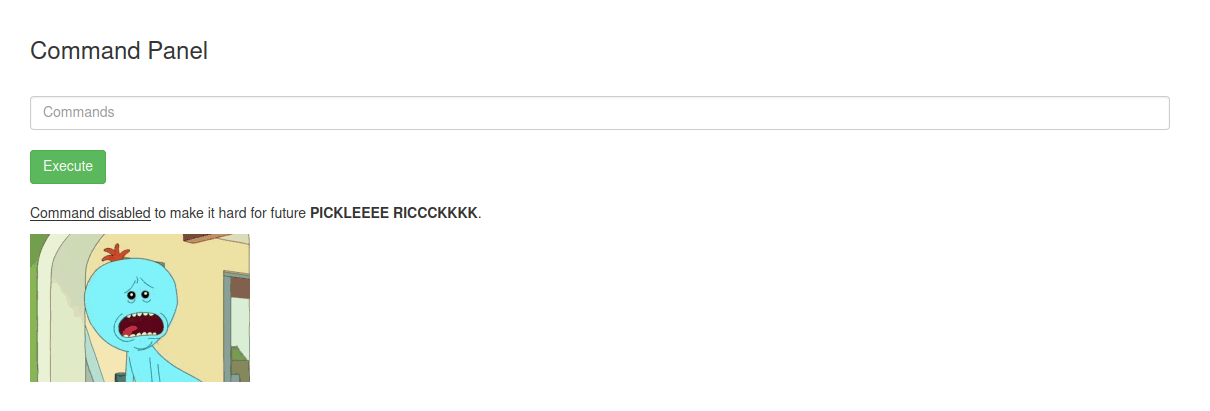
\includegraphics[width=\textwidth]{Complete_Beginner_Path/Web_Hacking_Fundamentals_Room/PickleRick/ErrorMsg.png}
So we have to try to find an equivalent command to find these contents and resort to \cd{less}.\\
This is successful and we see its contents:\\
\F{mr. meeseek hair}
We further know that the \cd{less} command works to show the contents of text files, so we look at the \cd{clue.txt} and read: 
\cdnl{Look around the file system for the other ingredient.}
Following this advice we try to get out of our current working directory, \cd{/var/www/html}, so we start lsiting the contents of everything we find on our way up via \cd{ls -la ../../../} until we arrive at the parent directory, where we find a \cd{/home} subdirectory containing a \cd{/rick} folder that looks very promising, and inside we find the file \cd{second ingredient}, and after printing it via \cdnl{less ../../../home/rick/``second ingredient''} we see the second ingredient is 
\F{1 jerry tear}

Now we don`t know how to keep going on, so we try to know how far we can escalate our privileges via \cd{sudo -l} and see we can execute all commands as sudo:
\cdnl{User www-data may run the following commands on ip-10-10-127-149.eu-west-1.compute.internal:\\
    (ALL) NOPASSWD: ALL} 
    
Seeing we have sudo permissions we can run the command \cd{sudo ls -lah /root} and there we find the 3rd ingredient under \cd{3rd.txt}:
\F{3rd ingredients: fleeb juice}
Hence we are done with this and can terminate the machine.\\


Again as a recapitulation:\\
We caught this flag by taking the following steps:
\label{Stepwise_WriteUp_Web_Hacking}
\begin{enumerate}
\item Run an gobuster scan on the target enumerating directories.
\item Run an Nmap scan on the target (in this case with \cd{-A, -p-} switches activated.
\item Look at the page's source code and search for vulnerabilities and possible Security Misconfiguration vulnerabilities.
\item Run a new gobuster scan with the most common extensions, such as .txt, .html, .php, .pdf, .css, .js, etc.
\item Read through all newly discovered files.
\item Try the found possible credentials on the login, or attempt a Bruteforce login on the page using Burp
\item When finding a command line, try to further enumerate the system. If some commands are blocked, try to find similar alternatives.
\item After enumerating as far as we can within the current user, we try to find sudo permissions using \cd{sudo -l}
\item We escalate as high as we can and try to further enumerate folders.
\end{enumerate}